\documentclass[a4paper, 11pt, twoside]{book}
\usepackage[a4paper]{geometry}
\usepackage{textcomp}
\usepackage{color}
\usepackage{url}
\usepackage{amsfonts}
\usepackage{float}
\usepackage{booktabs}
\usepackage{longtable}
\usepackage{makeidx}
\usepackage{fancyhdr}
\usepackage[times]{quotchap}
\usepackage{amsmath}
\usepackage{listings}
\usepackage{fancybox}
\usepackage{enumitem}

%% Aggiunge una linea al di sotto di ogni sezione principale
\usepackage[calcwidth]{titlesec}
\titleformat{\section}[hang]{\sffamily\bfseries}
 {\Large\thesection}{12pt}{\Large}[{\titlerule[0.4pt]}]

%% Gestisce la grafica a seconda che si usi latex o pdflatex
\newif\ifpdf
\ifx\pdfoutput\undefined
\pdffalse % no pdflatex
\else
\pdfoutput=1 % pdflatex
\pdftrue
\fi
%
\ifpdf
\usepackage[pdftex]{floatflt,graphicx}
\DeclareGraphicsExtensions{.pdf,.mps,.png,.jpg}
\usepackage[hidelinks,pdftex]{hyperref}
\else
\usepackage{floatflt,graphicx}
\DeclareGraphicsExtensions{.eps}
\fi
\usepackage{subfig}
\usepackage{adjustbox}
\usepackage{multirow}

\usepackage{algorithm}
\usepackage{algorithmic}
\usepackage[utf8]{inputenc} % per accenti

%%%%%%%%%%%%% NUOVI COMANDI E IMPOSTAZIONI %%%%%%%%%%%
\newenvironment{mcquote}
  {\begin{list}{}{
      \setlength{\rightmargin}{\leftmargin}}
         \item[]``\ignorespaces}
  {\unskip''\end{list}}
  
\newcommand{\mcchap}[2]{\protect{
 \chapter{#1}
 \label{#2}
}}

%% Gestione header: no header sulle dispari bianche
\makeatletter
\def\cleardoublepage{\clearpage\if@twoside \ifodd\c@page\else%
    \hbox{}%
    \thispagestyle{empty}%              % Empty header styles
    \newpage%
    \if@twocolumn\hbox{}\newpage\fi\fi\fi}
\makeatother

\makeatletter
\newenvironment{CenteredBox}{% 
\begin{Sbox}}{% Save the content in a box
\end{Sbox}\centerline{\parbox{\wd\@Sbox}{\TheSbox}}}% And output it centered
\makeatother
\usepackage[nottoc,numbib]{tocbibind}
\makeindex
\linespread{1.1}
\floatname{algorithm}{Algoritmo}
\renewcommand{\listalgorithmname}{Elenco degli algoritmi}

\newcommand{\placetextbox}[3]{% \placetextbox{<horizontal pos>}{<vertical pos>}{<stuff>}
  \setbox0=\hbox{#3}% Put <stuff> in a box
  \AddToShipoutPictureFG*{% Add <stuff> to current page foreground
    \put(\LenToUnit{#1\paperwidth},\LenToUnit{#2\paperheight}){\vtop{{\null}\makebox[0pt][c]{#3}}}%
  }%
}%


%%%%%%%%%%%%%%%% METADATI DOCUMENTO %%%%%%%%%%%%%%%%%%
\date{}

%%%%%%%%%%%%%%%%%% INIZIO DOCUMENTO %%%%%%%%%%%%%%%%%%
\begin{document}
\pagestyle{empty}

%% Pagina del titolo
  \begin{titlepage}
  \begin{center}
  \begin{large}
  {\fontsize{20}{18}\selectfont\vspace*{0.50cm}Università dell'Insubria}\\
  \vspace{.1cm}
  Dipartimento di Scienze Teoriche e Applicate - DiSTA\\
  \vspace{.1cm}
  Corso di Laurea Triennale in Informatica
  \end{large}
  
  \vspace{1cm}
  \begin{figure}[h]
    \begin{center}
      
\includegraphics[scale=0.16]{figure/insubria.png}
    \end{center}
  \end{figure}

    {\fontsize{25}{25}\usefont{OT1}{phv}{bc}{n}\selectfont\par
    Dashboard per COVID-19}
    \par    
    \vspace{2.4cm}
    \begin{large}
    Tesi di:\\
    Alessandro Riva\\
    Matricola 734572\\
    \vspace{2.3cm}
    Relatore:\\
    Prof. Davide Tosi\\
    \vfill
    Marzo, 2021
    \end{large}
    

  \end{center}
\end{titlepage}
  \cleardoublepage{}
  ~\\
~\\
~\\
~\\
~\\
~\\
~\\
~\\
~\\
~\\
~\\
~\\
~\\
~\\
~\\
~\\
~\\
~\\
~\\
~\\
~\\
~\\
~\\
~\\
~\\
~\\
~\\
~\\
~\\
~\\
~\\
~\\
~\\
\begin{flushright}
\emph{Per questo traguardo devo ringraziare innanzitutto i miei genitori, che mi hanno sostenuto e incoraggiato durante questi anni. Senza mia madre e mio padre, non avrei avuto la possibilità di studiare e di scrivere questo elaborato.}
\end{flushright}
  
%% Indice ed elenchi  
  \pagenumbering{roman}
  \setcounter{page}{1}
  \setcounter{tocdepth}{3}
  \renewcommand*\contentsname{Contenuti}
  \tableofcontents
  
%% Inizio capitoli
  \mainmatter{}

%% Capitoli
  \pagestyle{fancy}
  \renewcommand{\chaptermark}[1]{\markboth{#1}{}} 
  \renewcommand{\sectionmark}[1]{\markright{\thesection\ #1}} 
  \fancyhf{} % delete current setting for header and footer 
  \fancyhead[LE,RO]{\bfseries\thepage} 
  \fancyhead[LO]{\bfseries\rightmark} 
  \fancyhead[RE]{\bfseries\leftmark} 
  \renewcommand{\headrulewidth}{0.8pt} 
  \renewcommand{\footrulewidth}{0pt} 
  %\renewcommand{\headheight}{13.59999pt}
  \addtolength{\headheight}{0.5pt} % make space for the rule 
  \fancypagestyle{plain}{% 
  \fancyhead{} % get rid of headers on plain pages
  \fancyfoot[C]{\bfseries \thepage}
  \renewcommand{\headrulewidth}{0pt} % and the line 
  } 

\cleardoublepage{}
\setcounter{page}{1}
\mcchap{Introduzione}{cap:intro}


Viviamo in un mondo sempre più data-driven. La quantità di dati prodotti ogni giorno cresce in modo esponenziale.
I dati sono fondamentali per prendere decisioni in modo 



Giornalmente il dipartimento di Protezione Civile comunica comunica i dati relativi alla pandemia di Covid 19, per una migliore consultazione di tali dati si è pensato di sviluppare un’applicazione in grado di trasformarli automaticamente in grafici per una più facile lettura e comprensione dell’andamento della pandemia.
Lo scopo del seguente elaborato è quello di descrivere la struttura dell'applicazione creata per la realizzazione di questo servizio posto online, attraverso l’elaborazione dei dati relativi all’emergenza di Coronavirus Covid-19 utilizzando dei grafici interattivi.

\mcchap{Conclusioni}{cap:conclusion}
\chapter*{Colophon}

The \LaTeX~template for this thesis was made by Carullo Moreno.\\
\mcchap{Manuale utente}{cap:manuale}

\section{Esecuzione in locale}

\subsection{Requisiti software}
Il progetto è stato realizzato utilizzando \emph{ambiente di sviluppo integrato} (IDE) Pycharm Community.
Per l'esecuzione della dashboard sono richieste le seguenti dipendenze.
\begin{itemize}
 \item Git
 \item Python 3.8.5
 \item Pandas
 \item Plotly 
 \item Dash 
 \item Dash Bootstrap Components
 \end{itemize}
 
 \subsection{Clonazione del repository}
 E' possibile scaricare il progetto direttamente dal mio repository Github, con il comando \texttt{git clone https://github.com/alex27riva/Covid-dashboard}
 
 \subsection{Installazione dipendenze}
 Per installare le librerie richieste è sufficiente lanciare i seguenti comandi dal termianle integrato in Pycharm.
 
 \begin{itemize}
     \item \texttt{\$ pip install pandas}
     \item \texttt{\$ pip install plotly==4.12.0}
     \item \texttt{\$ pip install dash==1.17.0}
     \item \texttt{\$ pip install dash-bootstrap-components}
 \end{itemize}
 
 \begin{figure}[htp]
    \centering
    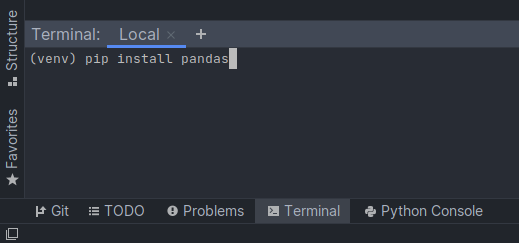
\includegraphics[width=10cm]{pycharm_terminal}
    \caption{Terminale integrato in Pycharm}
    \label{fig:pycharm_termianl}
\end{figure}

Ad installazione completata, sarà possibile avviare il progetto.

\subsection{Avvio del programma}

Per avviare il programma basta premere sul pulsante con la freccina verde.
Verrà avviato un server locale, il cui suo URL verrà mostrato nella console di debug a cui si potrà visualizzare la pagina della dashboard.

 \begin{figure}[htp]
    \centering
    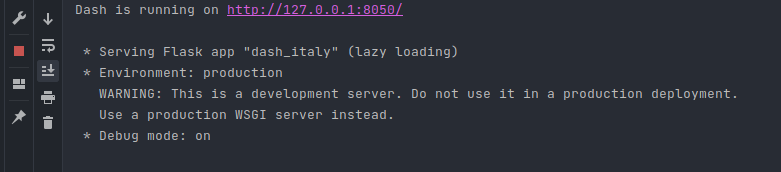
\includegraphics[width=9cm]{running_program}
    \caption{Programma Python in esecuzione}
    \label{fig:running_program}
\end{figure}

\section{Configurazione della VPS}
E' necessario disporrre di un server privato virtuale (VPS) con sistema operativo Ubuntu Server.

\subsection{Creazione account utente}
Per questioni di sicurezza è meglio non utilizzare l'account privilegiato \emph{root}.
\begin{enumerate}
\item Collegarsi alla VPS tramite SSH \texttt{ssh root@<ip-della-VPS>}
\item Crea l'account per l'utente admin \texttt{useradd -m admin}
\item Imposta una password per l'utente admin \texttt{passwd admin}
\item Chiudi la connessione con il comando \texttt{exit}
\end{enumerate}

\subsection{Installazione di Docker}

\begin{enumerate}
\item Collegati alla VPS con l'account admin \texttt{ssh admin@<ip-della-VPS>}
\item Scarica lo script per l'installazione di Docker \texttt{curl -fsSL https://get.docker.com -o get-docker.sh}
\item Esegui lo script con \texttt{sudo sh get-docker.sh}
\item Esegui questo comando per interagire con Docker senza previlegi di root \texttt{sudo usermod -aG docker admin}
\end{enumerate}

\subsection{Installazione e avvio dei container}
I container con le tre dashboard sono presenti nei repository di Docker, è sufficiente eseguire i seguenti comandi per la loro installazione e avvio.
\begin{itemize}
\item \texttt{docker run -d -p 8050:8050 --name=dashboard\_italy alex27riva/dash\_italy}
\item \texttt{docker run -d -p 8051:8050 --name=dashboad\_lomb alex27riva/dashboard\_lombardia}
\item \texttt{docker run -d -p 8052:8050 --name=dashboard\_regioni alex27riva/dashboard\_regioni}
\end{itemize}

\subsection{Portainer}
Per una gestione più semplice dei container Docker è possibile installare Portainer, un interfaccia web che facilita l'avvio, aggiornamento, rimozione dei container.
Per installare Portainer sono necessari questi due comandi:
\begin{enumerate}
    \item \texttt{docker volume create portainer\_data}
    \item \texttt{docker run -d -p 8000:8000 -p 9000:9000 --name=portainer --restart=always\\ -v /var/run/docker.sock:/var/run/docker.sock -v portainer\_data:/data\\ portainer/portainer-ce}
\end{enumerate}

Ora si può collegarsi all'interfaccia web all'indirizzo \emph{http://\textless ip-vps\textgreater:9000}

\subsection{Ngnix}
Ngnix è un web server, che è stato utilizzato come reverse proxy.

\subsubsection*{Installazione di Ngnix}

\begin{enumerate}
    \item \texttt{sudo apt update}
    \item \texttt{sudo apt install nginx}
    \item \texttt{unlink /etc/nginx/sites-enabled/default}
    \item \texttt{sudo nano /etc/nginx/sites-available/reverse-proxy.conf}
\end{enumerate}

\begin{lstlisting}[basicstyle=\ttfamily\small]
server
 {
    listen 80;
    listen 443;
    listen [::]:80;
    ssl on;
    ssl_certificate /etc/letsencrypt/live/dash.covid19-italy.it/fullchain.pem;
    ssl_certificate_key /etc/letsencrypt/live/dash.covid19-italy.it/privkey.pem;

    server_name dash.covid19-italy.it
    
    access_log /var/log/nginx/reverse-access.log;
    error_log /var/log/nginx/reverse-error.log;
    
    location /italy/ {
                proxy_pass http://localhost:8050;

    }

    location /lombardy/ {
            proxy_pass http://localhost:8051;

    }

    location /regions/ {
            proxy_pass http://localhost:8052;

    }
}
\end{lstlisting}

\subsubsection*{Creazione del link simbolico}
\texttt{\$ ln -s /etc/nginx/sites-available/reverse-proxy.conf\\ /etc/nginx/sites-enabled/reverse-proxy.conf}

\subsubsection*{Test della configurazione}
\texttt{nginx -t}

\subsection*{Installazione certificato SSL}
\begin{enumerate}
\item Assicurarsi che snap sia aggiornato \texttt{sudo snap install core; sudo snap refresh core}
\item Installare Certbot \texttt{sudo snap install --classic certbot}
\item Crea link simbolico per l'eseguibile \texttt{sudo ln -s /snap/bin/certbot /usr/bin/certbot}
\item Richiesta del certificato \texttt{sudo certbot --nginx}
\end{enumerate}

\subsection{riavvio di Nginx}
Riavviare il servizio di Nginx con il seguente comando: \\
\texttt{sudo systemctl restart nginx}


  
\appendix
\backmatter{}
\printindex

\bibliographystyle{biblio/IEEEtran}
\bibliography{biblio/egbib}
   
\end{document}